\section{Work Profiling}\label{sec:prof}

In this section, we describe how to measure work online. Total work is just the sum of the costs of all executed basic blocks, so it is
possible to embed its computation into the execution of the program. A na\"{\i}ve instrumentation would use a global counter initialized 
to zero. Each basic block would then have only to increment this counter with the total cost of its
instructions every time it is executed. Although easy to implement, the na\"{\i}ve approach introduces a significant overhead.

Previous work on basic block profiling has proposed optimal ways for instrumenting the code with as little overhead as possible without
losing any profiling information~\citep{knuth73,ball94}. The underlying idea is to instrument only a subset of the basic blocks of a
function and use the function's control flow graph (CFG) to calculate execution counts for the rest. We can use the same idea for our
purposes. Work profiling and basic block profiling are similar, both need to count how many times each basic block was executed. The only
important difference is that we do not have to store the execution count of each basic block, only the total work.

Graph theory shows that we can calculate precisely the frequencies of all edges between basic blocks if we choose a spanning tree of the
function CFG and instrument the edges in the complement of the spanning tree~\cite{nahapetian73,forman81}.
To make the instrumentation probe placement optimal, we choose the maximum spanning tree,
with the edge weights representing edge frequency estimates. By doing so, we leave as many high frequency edges as possible in the
maximum spanning tree and they will not be instrumented, allowing us to minimize the instrumentation overhead~\cite{forman81,ball94}.

\begin{figure}[t]
\centering {
  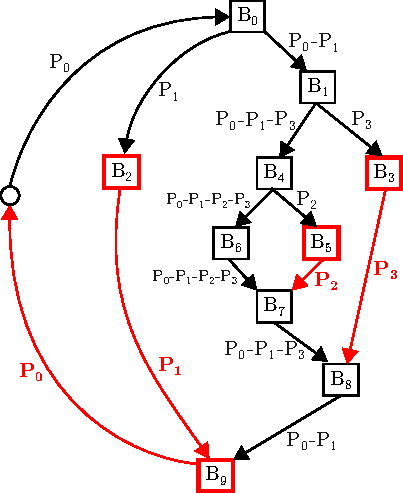
\includegraphics[scale=0.75]{figs/cfg-example.pdf}\\\vspace{1ex}
  \resizebox{0.45\textwidth}{!}{
  %\scalebox{0.8}{
     \begin{minipage}{0.5\textwidth}
     Instrumented value for each probe $P_i$:
     \begin{align*}
     \omega(P_0) &= w(B_0) + w(B_1) + w(B_4) + w(B_6) + w(B_7) + w(B_8) + w(B_9)\\
     \omega(P_1) &= w(B_2) - w(B_1) - w(B_4) - w(B_6) - w(B_7) - w(B_8)\\
     \omega(P_2) &= w(B_5) - w(B_6)\\
     \omega(P_3) &= w(B_3) - w(B_4) - w(B_6) - w(B_7)
     \end{align*}
     \end{minipage}
  }
}
  \caption{Example of a CFG with its maximum spanning tree in black. Basic blocks and edges highlighted in red are instrumented.
    Instrumenting them is enough for calculating the total work performed by the whole CFG.}
  \label{fig:cfg-example}
\end{figure}

In contrast to the naive instrumentation where each basic block records only its own amount of work, with the optimal profiling the work
counter increments needs to take other basic blocks into account. Figure~\ref{fig:cfg-example} shows an example CFG, where the instrumented
blocks are marked with red. In this example, executing block $B_5$ implies not executing $B_6$. To compute the amount of work associated
with each instrumentation probe, we first need to determine how reaching a probe relates with executing or not a basic block. Starting from
instrumented edges, we build symbolic expressions for each edge of their frequency counts as a linear function of probe counts, as seen in
Figure~\ref{fig:cfg-example}. If a symbolic expression for an edge and the corresponding block contains a positive term for a probe, this
means that the block is executed when we reach the probe, so the block's cost should be added at that probe. Conversely, if the expression
contains a negative term for a probe, then the block is executed when we do not reach the probe, so the block's cost should be subtracted.
In our example CFG, the symbolic expression for the basic block $B_8$ is $P_0 - P_1$, so the amount of work of $B_8$, denoted by $w(B_8)$,
is incremented in probe $P_0$ and decremented in $P_1$.

\paragraph{Populating the edge flows:}
Intuitively, if all the edge flows are known for the complement of a spanning tree then at any leaf of the spanning tree there is only one
unknown edge flow. This unknown edge flow can be calculated by Kirchhoff's first law\cite{knuth73,ball94},
also known as the principle of \textit{conservation of flow}, which states that
the amount of flow into a vertex equals the amount of output flow.
This process repeats as a bottom-up propagation until all the unknown edge flows have been calculated. This algorithm can be formally defined as a post-order traversal on the
spanning tree. Let $G$ be the CFG. This algorithm first initializes the edge flows $D_{(u,v)}$, for each edge $(u,v)$ in the CFG, as
follows:
\[
D_{(u,v)} \gets
\begin{cases}
    P_{(u,v)} & \quad \text{if edge $(u,v)$ has a probe $P_{(u,v)}$}\\
    0       & \quad \text{otherwise}
\end{cases}
\]
This initialization represents only the trivially known edge flows, which are the
probes themselves (the highlighted edges in red).

Afterwards, the algorithm consists in propagating the known edge flows, infering
the symbolic expressions in the unknown edge flows.
This is achieved by performing a bottom-up propagation from the trivially known
edge flows (in red) by applying the Kirchhoff's first law, i.e.,
for each vertex with a single unknown edge flow, we compute the difference between
the known incoming edge flows by the known outgoing edge flows.
Formally,
for each vertex $u\in G$, in a post-order traversal of the spanning tree,
we can use the Kirchhoff's first law and apply the following operations
in a symbolic fashion:
\[
\Sigma^+_u = \sum_{v\in N^+(u)} D_{(u,v)}
\]
\[
\Sigma^-_u = \sum_{v\in N^-(u)} D_{(v,u)}
\]
\[
\forall v\in N^+(u):  D_{(u,v)} \gets
\begin{cases}
    D_{(u,v)} & \quad \text{if $D_{(u,v)}\neq 0$}\\
    \Sigma^-_u - \Sigma^+_u       & \quad \text{otherwise}
\end{cases}
\]
\[
\forall v\in N^-(u):  D_{(v,u)} \gets
\begin{cases}
    D_{(v,u)} & \quad \text{if $D_{(v,u)}\neq 0$}\\
    \Sigma^+_u - \Sigma^-_u       & \quad \text{otherwise}
\end{cases}
\]

\paragraph{Composing the aggregated value of the probes:}
If $x$ is a symbolic expression, then $\kappa_P(x)$ represents the coefficient
of the term $P$ in $x$.
In our case, $\kappa_P(x)$ will belong to the set $\{-1,0,1\}$.
Then, for all probes $P$:
\[
\omega(P) = \sum_{u\in G} \kappa_P(\Sigma^+_u)w(u)
\]

\subsection{Relaxed Instrumentation}

Optimal instrumentation significantly reduces the profiling overhead when compared to naive instrumentation, from an average overhead of
79\% to 13\%. In some extreme cases though optimal instrumentation can result in overheads of up to 60\% (see benchmark \texttt{adpcm\_d}
in Figure~\ref{fig:overhead-O3}). To further reduce the overhead in these cases, we propose a relaxation strategy that offers a trade-off
between accuracy and overhead. While in traditional basic block profiling the aim is to accurately measure the frequency counts of every
single block, in our case we only care about the total amount of work. Our insight was that if the work associated with a probe is small,
then ignoring the probe will have little effect on the total work estimation. By removing such probes, especially if they are frequently
executed, we can reduce the instrumentation overhead dramatically.

Our relaxation strategy operates on selection of probes and weights as decided by the optimal algorithm. Removing low weight probes is
easy, but we need a way to guarantee that the error in our work estimation will not grow too big. Our conservative approach, decides on an
upper bound for the error and applies it recursively on every loop of the CFG. Specifically, our algorithm extracts all subgraphs
representing loops and transforms them into DAGs (Directed Acyclic Graphs) by removing the backedge and moving inner loops into separate
DAGs. An example of this is shown in Figure~\ref{fig:cfg-relax-example}, where the CFG is partitioned into two DAGs.

%The relaxation starts by extracting DAGs from the CFG.
%First, the algorithm extracts all the subgraphs that represent a loop or the outer most region of the function.
%Afterwards, these subgraphs are transformed into DAGs by ignoring the backedge
%and also by considering that any loop within the subgraph is never executed,
%i.e., only the headers of the inner loops are actually included into the DAG.
%Figure~\ref{fig:cfg-relax-example} shows a CFG partitioned into two DAGs (consider
%only basic blocks and edges completely inside the yellow and green boundaries).

\begin{figure}[t]
  \centering
  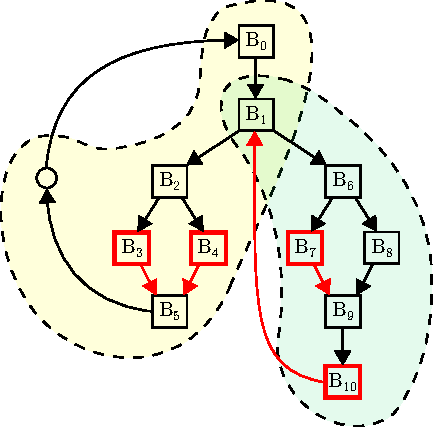
\includegraphics[scale=0.75]{figs/cfg-relax-example.pdf}
  \caption{Example of a CFG containing a loop and its decomposition into DAGs.
           The DAGs are the subgraphs within the dashed boundaries.}
  \label{fig:cfg-relax-example}
\end{figure}

%\begin{lstlisting}[caption={Optimal placement of probes for block frequency.}, label={lst:instrumentCFG}]
%// Input: CFG
%relaxInstrumentation(G) {
%  for loop in G:
%     DAG = colapseInnerLoops(loop)
%     relaxInstrumentedDAG(DAG)
%  DAG = colapseInnerLoops(G)
%  relaxInstrumentedDAG(DAG)
%}
%\end{lstlisting}

For every DAG with a set of probes $\{P_0, P_1, \ldots, P_k\}$, we calculate $m$, the minimum amount of work that can be performed in the
DAG. Given this, the worst case relative error caused by removing a probe $P_i$ is $\varepsilon(P_i) = \frac{\omega(P_i)}{m}$. Reducing the
instrumentation overhead as much as possible while keeping the total worst case error below a threshold can be modeled as a 0-1 Knapsack
problem:
\begin{gather*}
\textrm{max.}\quad\sum_{i=0}^{k} f(P_i)x_i,\quad
\textrm{s.t.}\quad\sum_{i=0}^{k} \varepsilon(P_i)x_i \leq M \\
x_i\in\{0,1\}, i\in\{0,\ldots,k\}
\end{gather*}
where $f(P_i)$ is the execution frequency of probe $P_i$ and $x_i$ denotes the probes selected for removal. By constraining the worst case
relative error in every single DAG of the CFG, we guarantee that the final error introduced by relaxation will always be below the chosen
threshold.
% Furthermore, by constraining the percentage error of every DAG below a given threshold, we guarantee that the final error of the relaxation will always be bounded by the threshold, as demonstrated by Proposition~\ref{prop:relax-bound}.
%
% \begin{prop}\label{prop:relax-bound}
% Let $n_i$ be the number of times a given DAG $i$ is executed, $r_i$ be the total relaxation (amount of work removed) in DAG $i$, and $m_i$ be its minimum amount of work.
% If $\frac{r_i}{m_i} \leq M$ for every $i$,
% then the final error of the relaxation will always be bounded by the same threshold.
% \end{prop}
% \begin{proof}
% We can model the overall error of the relaxation as:
% \[
% 1 - \frac{n_1(m_1 - r_1) + n_2(m_2 - r_2) + \ldots + n_k(m_k - r_k) + c}{n_1m_1 + n_2m_2 + \ldots + n_km_k + c}
% \]
% That is,
% %\begin{equation*}
% \begin{gather*}
%  1 - \frac{n_1m_1 + n_2m_2 + \ldots + n_km_k + c}{n_1m_1 + n_2m_2 + \ldots + n_km_k + c} + \frac{n_1r_1 + n_2r_2 + \ldots + n_kr_k}{n_1m_1 + n_2m_2 + \ldots + n_km_k + c} = \\
%  \frac{n_1r_1 + n_2r_2 + \ldots + n_kr_k}{n_1m_1 + n_2m_2 + \ldots + n_km_k + c}
% \end{gather*}
% %\end{equation*}
% If $\frac{r_j}{m_j}$ is the maximum ratio $\frac{r_i}{m_i}$ for every $i$, then
% \begin{equation*}
% \begin{aligned}
%  \frac{n_1r_1 + n_2r_2 + \ldots + n_kr_k}{n_1m_1 + n_2m_2 + \ldots + n_km_k + c} &\leq\\
%  \frac{n_1r_j + n_2r_j + \ldots + n_kr_j}{n_1m_j + n_2m_j + \ldots + n_km_j + c} &\leq\\
%  \frac{n_1r_j + n_2r_j + \ldots + n_kr_j}{n_1m_j + n_2m_j + \ldots + n_km_j} &
% \end{aligned}
% \end{equation*}
% If $N = max\{n_i$ for every $i\}$, then
% \begin{equation*}
% \begin{aligned}
%  \frac{n_1r_j + n_2r_j + \ldots + n_kr_j}{n_1m_j + n_2m_j + \ldots + n_km_j} &\leq\\
%  \frac{Nr_j + Nr_j + \ldots + Nr_j}{Nm_j + Nm_j + \ldots + Nm_j} &=\\
%  \frac{Nkr_j}{Nkm_j} = \frac{r_j}{m_j} &\leq M
% \end{aligned}
% \end{equation*}
% \end{proof}


%\begin{lstlisting}[caption={Optimal placement of probes for block frequency.}, label={lst:instrumentCFG}]
%// Input: CFG
%relaxInstrumentedDAG(DAG){
%   P = ProbesIn(DAG)
%   m = minWork(DAG,P)
%   K = createKnapsackModel(P,m)
%   Bag = solveKnapsack(K)
%   for B in (P-Bag):
%     removeProbe(B)
%}
%\end{lstlisting}

%The necessary block-frequency information for optimising both the placement of
%probes can be acquired from profiles of previous executions of the program or by
%a static heuristic of the CFG during compilation.

For our experiments, we implemented two solvers for the 0-1 Knapsack problem: an optimal but potentially slow brute-force solver and a
greedy heuristic based on sorting the items~\citep{dantzig57}. We use the brute-force solver for DAGs with a small number of probes, the
greedy heuristic otherwise.

\subsection{Whole Program Relaxation}

The proposed relaxation strategy provides hard guarantees that error will remain below the chosen threshold but in many cases these
guarantees are too conservative. Our worst case scenario approach assumes that each loop will always perform the minimum amount of work
possible which might be orders of magnitude less than the work actually performed. In such cases, we remove too few probes and have little
effect on the instrumentation overhead, while the actual relative error in our work estimation is negligible. To avoid this problem, we
propose an adapted version of the relaxation algorithm that operates on the whole program.

\textit{Whole program relaxation} works by using block-frequency profiling from previous executions. With this information, we are able to
compute the error of removing a given probe in terms of the whole program's execution, and then select a subset of all the probes to be
removed.

For a program with a set of probes $\{P_0, P_1, \ldots, P_k\}$, we model the whole program relaxation as the following 0-1 Knapsack
problem:
\begin{gather*}
\textrm{max.}\quad\sum_{i=0}^{k} f(P_i)x_i,\quad
\textrm{s.t.}\quad\sum_{i=0}^{k} \varepsilon(P_i)x_i \leq M \\
x_i\in\{0,1\}, i\in\{0,\ldots,k\}
\end{gather*}
where $f(P_i)$ is the execution frequency of the instrumented basic block $P_i$, $x_i$ denotes the probes selected for removal, $M$ is the
error threshold, and $\varepsilon(P_i)$ is the error of removing probe $P_i$ relative to the total work.
%if $\Delta W$ is the work
%value for the whole program's execution, computed from the basic block frequencies profiled from previous executions, the error for a
%given probe $P_i$ is
%\[
%\varepsilon(P_i) = \frac{\omega(P_i)f(P_i)}{\Delta W}.
%\]

Contrary to the per DAG relaxation, the error introduced by whole program relaxation is not guaranteed to be bounded by the error threshold
$M$. Still, we expect it to remain close to the threshold as long as the program's behavior does not deviate significantly from the
behavior captured in profile we used.
